\documentclass[13pt]{beamer}
%
% Choose how your presentation looks.
%
% For more themes, color themes and font themes, see:
% http://deic.uab.es/~iblanes/beamer_gallery/index_by_theme.html
%
\mode<presentation>
{
\usetheme{CambridgeUS}     % or try Darmstadt, Madrid, Warsaw, ...
\usecolortheme{beaver} % or try albatross, beaver, crane, ...
\usefonttheme{default}  % or try serif, structurebold, ...
\setbeamertemplate{navigation symbols}{}
\setbeamertemplate{caption}[numbered]
} 

\usepackage[english]{babel}
\usepackage[utf8x]{inputenc}
\usepackage{xcolor}
\usepackage{multicol}
\usepackage{tikz}
\usepackage{tikz-uml}
\tikzumlset{font=\footnotesize\ttfamily}
\usepackage{hyperref}

\usepackage{listings}
\definecolor{codegreen}{rgb}{0,0.6,0}
\definecolor{codegray}{rgb}{0.5,0.5,0.5}
\definecolor{codepurple}{rgb}{0.58,0,0.82}
\definecolor{backcolour}{rgb}{0.95,0.95,0.92}

\lstdefinestyle{myCustomCppStyle}{
language=C++,
numbers=left,
stepnumber=1,
numbersep=9pt,
tabsize=2,
showspaces=false,
showstringspaces=false
}

\lstset{basicstyle=\tiny,style=myCustomCppStyle}

\lstdefinestyle{mystyle}{
backgroundcolor=\color{backcolour},   
commentstyle=\color{codegreen},
keywordstyle=\color{magenta},
numberstyle=\tiny\color{codegray},
stringstyle=\color{codepurple},
basicstyle=\ttfamily\footnotesize,
breakatwhitespace=false,         
breaklines=true,                 
captionpos=b,                    
keepspaces=true,                 
numbers=left,                    
numbersep=5pt,                  
showspaces=false,                
showstringspaces=false,
showtabs=false,                  
tabsize=1
}

\lstset{style=mystyle}

\usepackage{graphicx}
\graphicspath{ {./images/} }

\usepackage{tikz}
\usetikzlibrary{decorations.text}
\usetikzlibrary{shapes.geometric, arrows, positioning, calc, matrix}

\tikzset{
basic box/.style={
shape=rectangle, rounded corners, align=center,
draw=#1, fill=#1!25},
header node/.style={
Minimum Width=header nodes,
font=\strut\Large\ttfamily,
text depth=+0pt,
fill=white, draw},
header/.style={
inner ysep=+1.5em,
append after command={
\pgfextra{\let\TikZlastnode\tikzlastnode}
node [header node] (header-\TikZlastnode) at (\TikZlastnode.north) {#1}
node [span=(\TikZlastnode)(header-\TikZlastnode)] at (fit bounding box) (h-\TikZlastnode) {}
}
},
hv/.style={to path={-|(\tikztotarget)\tikztonodes}},
vh/.style={to path={|-(\tikztotarget)\tikztonodes}},
fat blue line/.style={ultra thick, blue}
}

\definecolor{mygray}{RGB}{208,208,208}
\definecolor{mymagenta}{RGB}{226,0,116}
\newcommand*{\mytextstyle}{\sffamily\Large\bfseries\color{black!85}}
\newcommand{\arcarrow}[3]{%
% inner radius, middle radius, outer radius, start angle,
% end angle, tip protusion angle, options, text
\pgfmathsetmacro{\rin}{1.7}
\pgfmathsetmacro{\rmid}{2.2}
\pgfmathsetmacro{\rout}{2.7}
\pgfmathsetmacro{\astart}{#1}
\pgfmathsetmacro{\aend}{#2}
\pgfmathsetmacro{\atip}{5}
\fill[mygray, very thick] (\astart+\atip:\rin)
             arc (\astart+\atip:\aend:\rin)
-- (\aend-\atip:\rmid)
-- (\aend:\rout)   arc (\aend:\astart+\atip:\rout)
-- (\astart:\rmid) -- cycle;
\path[
decoration = {
text along path,
text = {|\mytextstyle|#3},
text align = {align = center},
raise = -1.0ex
},
decorate
](\astart+\atip:\rmid) arc (\astart+\atip:\aend+\atip:\rmid);
}
\title[Design Pattern]{Structural Design Pattern}
\author{Hung Tran}
\institute{Fpt software}
\date{\today}


\begin{document}

\begin{frame}
	\titlepage
\end{frame}

\begin{frame}{Outline}
	\tableofcontents
\end{frame}

\section{Structural Pattern Overview}

\begin{frame}{Structural Pattern Overview}
	\begin{center}
		\textcolor{blue}{\textbf{How classes and objects are composed to form larger structure.}}
	\end{center}
	\begin{itemize}
		\item \textbf{Adapter}: Convert the interface of a class into another interface.
		\item \textbf{Bridge}: Decouple an abstraction from its implementation.
		\item \textbf{Composite}: Compose objects into tree structure.
		\item \textbf{Decorator}: Attach additional responsibilities to an object dynamically.
		\item \textbf{Facade}: Provide a unified interface to a set of interfaces.
		\item \textbf{Flyweight}: Use sharing to support large numbers of fine-grained objects efficiently.
		\item \textbf{Proxy}: Provide a surrogate or placeholder for another object to control access to it.
	\end{itemize}
\end{frame}

\section{Composite design pattern}

\begin{frame}{Problem Statement}
	\begin{columns}[T]
		\begin{column}{.45\textwidth}
			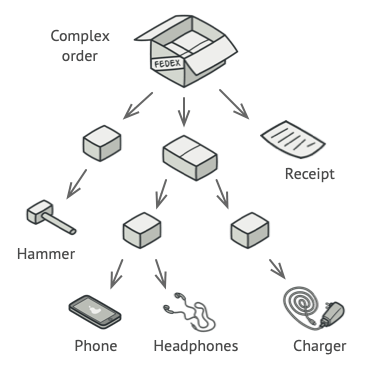
\includegraphics[scale=0.4]{./images/problem.png}
		\end{column}
	
		\begin{column}{.45\textwidth}
			\begin{itemize}
				\item Imagine that you have two types of objects: \textbf{Products} and \textbf{Boxes}
				\item A Box can contain several Products as well as a number of smaller Boxes.
				\item These little Boxes can also hold some Products or even smaller Boxes, and so on.
			\end{itemize}
		\end{column}
	\end{columns}
\end{frame}

\begin{frame}{Problem Statement}
	\begin{itemize}
		\item Create an ordering system that uses these classes
		\item Orders could contain simple products without any wrapping, as well as boxes stuffed with products...and other boxes.
		\item \textcolor{red}{How would you determine the total price of such an order?}
		\item You could try the direct approach: unwrap all the boxes, go over all the products and then calculate the total.
		\item That would be doable in the real world; but in a program, it’s not as simple as running a loop.
		\item You have to know the classes of Products and Boxes you’re going through, the nesting level of the boxes and other nasty details beforehand.
		\item All of this makes the direct approach either too awkward or even impossible.
	\end{itemize}
\end{frame}

\begin{frame}{The Intent of Composite Design Pattern}
	\begin{center}
	\textcolor{red}{\textbf{Compose objects into tree structures to represent part-whole hierarchies. Composite lets clients treat individual objects and compositions of objects uniformly.}}
	\end{center}
\end{frame}

\begin{frame}{Structure of Bridge Pattern: Object adapter}
	\begin{center}
		\begin{tikzpicture}
			\umlemptyclass[x=0,y=0]{Client}
			\umlclass[x=7,y=0]{Component}{}{operation()\\add()\\remove()\\getChild(int)}
			\umlclass[x=5,y=-4]{Leaf}{}{operation()}
			\umlclass[x=9,y=-4]{Composite}{}{operation()\\add()\\remove()\\getChild(int)}
			\umluniassoc[pos=0.95, align=right, name=uniassoc]{Client}{Component}
			\umlinherit[geometry=-|]{Leaf}{Component}
			\umlinherit[geometry=-|]{Composite}{Component}
			\umluniaggreg[geometry=|-]{Composite}{Component}
		\end{tikzpicture}	
	\end{center}
\end{frame}

\begin{frame}{Tree implementation}
\begin{columns}[T]
\begin{column}{.45\textwidth}
\lstset{basicstyle=\tiny,style=myCustomCppStyle}
component.h
\lstinputlisting{./examples/tree/component.h}
\end{column}

\begin{column}{.45\textwidth}
\lstset{basicstyle=\tiny,style=myCustomCppStyle}
component.cpp
\lstinputlisting{./examples/tree/component.cpp}
\end{column}
\end{columns}
\end{frame}

\begin{frame}{Tree implementation}
\begin{columns}[T]
\begin{column}{.45\textwidth}
\lstset{basicstyle=\tiny,style=myCustomCppStyle}
leaf.h
\lstinputlisting{./examples/tree/leaf.h}
\end{column}

\begin{column}{.45\textwidth}
\lstset{basicstyle=\tiny,style=myCustomCppStyle}
leaf.cpp
\lstinputlisting{./examples/tree/leaf.cpp}
\end{column}
\end{columns}
\end{frame}

\begin{frame}{Tree implementation}
\begin{columns}[T]
\begin{column}{.45\textwidth}
\lstset{basicstyle=\tiny,style=myCustomCppStyle}
composite.h
\lstinputlisting{./examples/tree/composite.h}
\end{column}

\begin{column}{.45\textwidth}
\lstset{basicstyle=\tiny,style=myCustomCppStyle}
composite.cpp
\lstinputlisting{./examples/tree/composite.cpp}
\end{column}
\end{columns}
\end{frame}

\begin{frame}{Applicability}
	\begin{itemize}
		\item Make sure that the core model of your app can be represented as a tree structure. Try to break it down into simple elements and containers. Remember that containers must be able to contain both simple elements and other containers.
		\item Declare the component interface with a list of methods that make sense for both simple and complex components.
		\item Create a leaf class to represent simple elements. A program may have multiple different leaf classes.
		\item Create a container class to represent complex elements. In this class, provide an array field for storing references to sub-elements. The array must be able to store both leaves and containers, so make sure it’s declared with the component interface type.
		% While implementing the methods of the component interface, remember that a container is supposed to be delegating most of the work to sub-elements.
		\item Finally, define the methods for adding and removal of child elements in the container.
		% Keep in mind that these operations can be declared in the component interface. This would violate the Interface Segregation Principle because the methods will be empty in the leaf class. However, the client will be able to treat all the elements equally, even when composing the tree.
	\end{itemize}
\end{frame}

\begin{frame}{How to implement}
	\begin{itemize}
		\item \textcolor{blue}{Use the Composite pattern when you have to implement a tree-like object structure.}
		\item The Composite pattern provides you with two basic element types that share a common interface: simple leaves and complex containers. A container can be composed of both leaves and other containers. This lets you construct a nested recursive object structure that resembles a tree.
		\item \textcolor{blue}{Use the pattern when you want the client code to treat both simple and complex elements uniformly.}
		\item All elements defined by the Composite pattern share a common interface. Using this interface, the client doesn’t have to worry about the concrete class of the objects it works with.
	\end{itemize}
\end{frame}

\begin{frame}{Pros and Cons}
\begin{columns}[T]
\begin{column}{.45\textwidth}
	\begin{itemize}
	\item You can work with complex tree structures more conveniently: use polymorphism and recursion to your advantage.
	\item Open/Closed Principle. You can introduce new element types into the app without breaking the existing code, which now works with the object tree.
	\end{itemize}
\end{column}

\begin{column}{.45\textwidth}
	\begin{itemize}
	\item It might be difficult to provide a common interface for classes whose functionality differs too much. In certain scenarios, you’d need to overgeneralize the component interface, making it harder to comprehend.
	\end{itemize}
\end{column}
\end{columns}
\end{frame}

\begin{frame}{Relations with Other Patterns}
	\begin{itemize}
		\item You can use Builder when creating complex Composite trees because you can program its construction steps to work recursively.
		\item Chain of Responsibility is often used in conjunction with Composite. In this case, when a leaf component gets a request, it may pass it through the chain of all of the parent components down to the root of the object tree.
		\item You can use Iterators to traverse Composite trees.
		\item You can use Visitor to execute an operation over an entire Composite tree.
		\item You can implement shared leaf nodes of the Composite tree as Flyweights to save some RAM.
		\item Composite and Decorator have similar structure diagrams since both rely on recursive composition to organize an open-ended number of objects.
		% A Decorator is like a Composite but only has one child component. There’s another significant difference: Decorator adds additional responsibilities to the wrapped object, while Composite just “sums up” its children’s results.
		
		%However, the patterns can also cooperate: you can use Decorator to extend the behavior of a specific object in the Composite tree.
		\item Designs that make heavy use of Composite and Decorator can often benefit from using Prototype.
		%Applying the pattern lets you clone complex structures instead of re-constructing them from scratch.
	\end{itemize}
\end{frame}

\begin{frame}
\begin{center}
{\fontsize{40}{50}\selectfont Thank You!}
\end{center}
\end{frame}

\end{document}
